\chapter{Sprint 3 : Sécurité, chiffrement et supervision}\label{chap6}

\section{Introduction}

Le troisième sprint renforce la confidentialité des données cliniques et la preuve d'intégrité. Chaque événement de traitement est chiffré avec une clé de données propre à l'épisode, puis son empreinte est inscrite dans deux chaînes de blocs et ancrée sur une chaîne EVM locale.

\section{Chiffrement enveloppe}

La Figure \ref{fig:envelope} présente le mécanisme de chiffrement. Une clé maître, fournie par l'environnement, dérive une clé d'encapsulation (KEK). Une clé de données (DEK) aléatoire est générée par épisode, encapsulée par la KEK et stockée dans \texttt{EpisodeKey}. La charge utile de l'événement est chiffrée avec la DEK puis conservée dans \texttt{Block.payload\_enc}.

\begin{figure}[H]
\centering
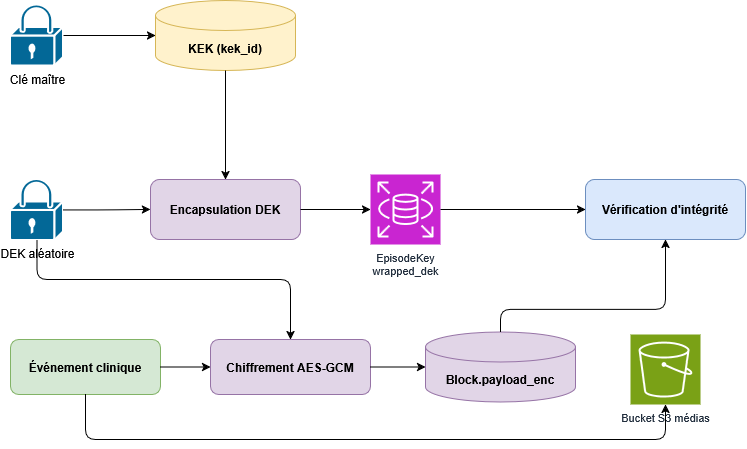
\includegraphics[width=\textwidth]{Chapters/6/images/10-chiffrement-enveloppe.png}
\caption{Flux de chiffrement enveloppe}
\label{fig:envelope}
\end{figure}

Cette conception permet de séparer les responsabilités : la base stocke des octets chiffrés, le fournisseur de clés reste externalisé, et la rotation de la clé maître peut être organisée sans réécrire les événements passés.

\section{Formation et ancrage des blocs}

La Figure \ref{fig:chain_seq} décrit la séquence complète. Après création de l'événement, le système calcule une empreinte et une racine Merkle, crée un bloc immuable dans la chaîne du patient ou du médecin, puis envoie le hash du bloc à Anvil. La transaction d'ancrage et le numéro de bloc sont conservés dans \texttt{Anchor}.

\begin{figure}[H]
\centering
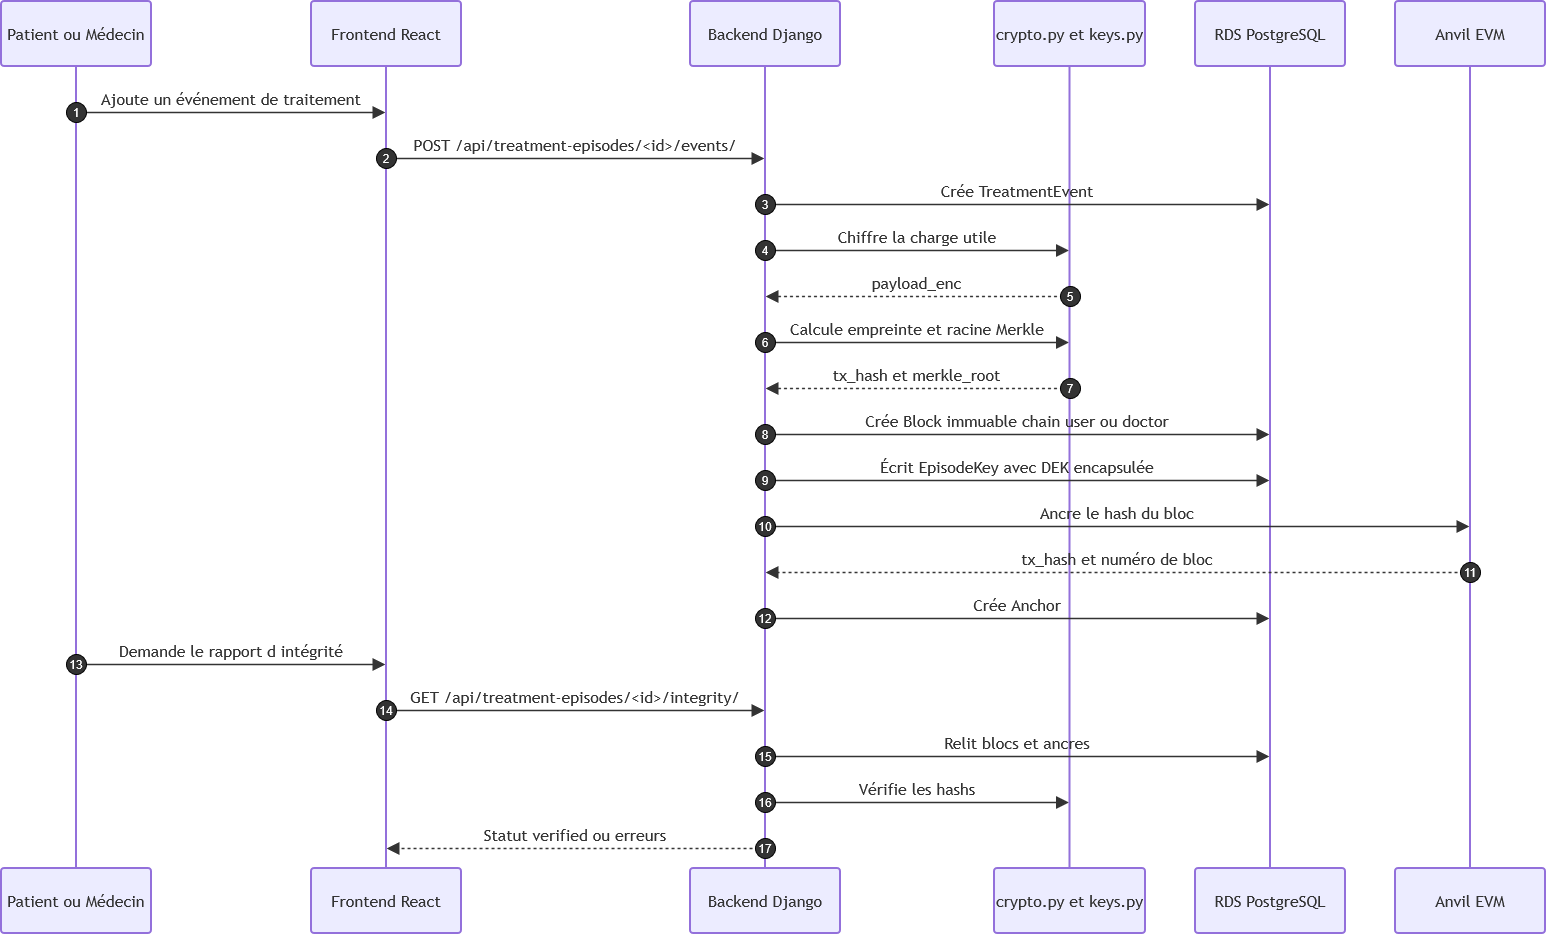
\includegraphics[width=\textwidth]{Chapters/6/images/09-integrite-blockchain-sequence.png}
\caption{Séquence d'intégrité et d'ancrage blockchain}
\label{fig:chain_seq}
\end{figure}

Le modèle \texttt{Block} interdit toute modification ou suppression : les méthodes \texttt{save} et \texttt{delete} lèvent une exception dès que l'objet possède une clé primaire. Les blocs sont organisés en deux chaînes par épisode, chacune avec un index unique et un hash du bloc précédent.

\newpage
\section{Supervision et journaux}

La Figure \ref{fig:logs} montre le pipeline de journalisation. Le backend émet des JSON structurés avec un identifiant \texttt{X-Request-ID}. Fluent Bit collecte ces flux, les enrichit et les envoie à Elasticsearch, où Kibana permet de construire des tableaux de bord et des alertes.

\begin{figure}[H]
\centering
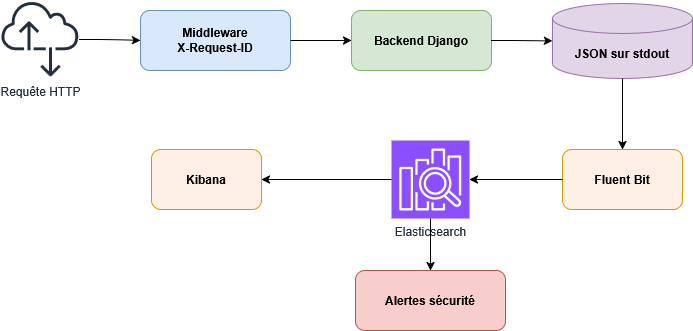
\includegraphics[width=\textwidth]{Chapters/6/images/11-pipeline-logs.png}
\caption{Pipeline de collecte et d'analyse des journaux}
\label{fig:logs}
\end{figure}

La Figure \ref{fig:audit} illustre la vue administrateur qui donne accès aux utilisateurs, aux alertes de sécurité et aux dernières activités.

\begin{figure}[H]
\centering
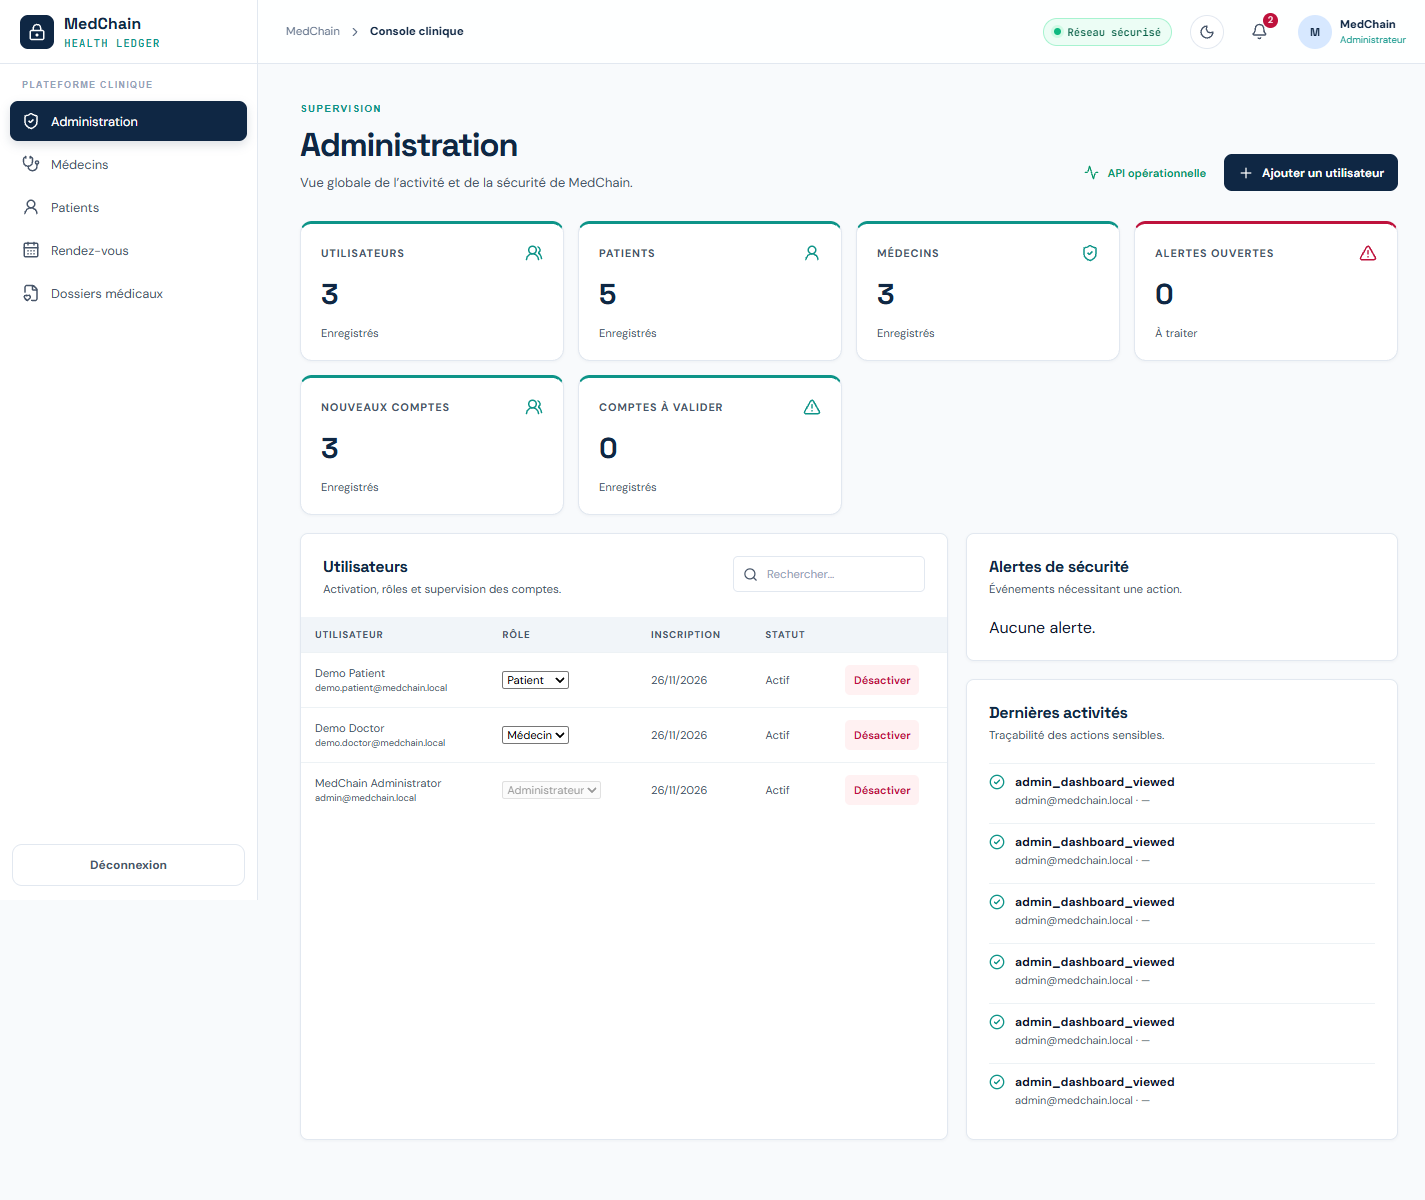
\includegraphics[width=\textwidth]{Images/Screenshots/S15-audit-et-alertes.png}
\caption{Journal d'audit et alertes de sécurité}
\label{fig:audit}
\end{figure}

\section{Conclusion}

Le volet sécurité est désormais complet : chiffrement des charges utiles, immutabilité des blocs, ancrage des empreintes et supervision des accès. Le dernier chapitre présente le déploiement et les résultats de validation.
